% !TEX root = LF-IMAPol.tex

\ohead{Writing conventions}

\chapter*{Writing conventions}
\addcontentsline{toc}{chapter}{Writing conventions}

\noindent
\begingroup
\setlength{\tabcolsep}{2.5pt}
\setlength\extrarowheight{3pt}
\small
\begin{longtable}{ l l >{\raggedright\arraybackslash}p{10cm} }

\multicolumn{3}{l}{{\large \textbf{Abbreviations}}} \\*[6pt]

$\mathcal{A}$ & \phantom{:} & a set of arcs in a network\slashs{}graph \\

\textsc{acc} & \phantom{:} & accusative case \\

Adj & \phantom{:} & Adjective \\

Adv & \phantom{:} & Adverb \\

A\tsub{(poss)} & \phantom{:} & possessive adjective (\textit{my}, \textit{your}, ...) \\

\textsc{art} & \phantom{:} & article or other determiner -- e.g. \textit{to have} \textsc{art} \textit{dream} \\

Claus & \phantom{:} & Clausative \\

\syntDname{circumst} & \phantom{:} & \syntDname{circumstantial} surface-syntactic relation \\

\textsc{dat} & \phantom{:} & dative case \\

\syntDname{determ} & \phantom{:} & \syntDname{determinative} surface-syntactic relation \\

\syntDname{dir-obj} & \phantom{:} & \syntDname{direct-objectival} surface-syntactic relation \\

DSynt- & \phantom{:} & deep-syntactic \\

DSyntA & \phantom{:} & deep-syntactic actant \\

DSyntS & \phantom{:} & deep-syntactic structure \\

%{\smaller Eng.} & \phantom{:} & English \\

\lf{f} & \phantom{:} & A given lexical function \\

\lfappl{f}{L} & \phantom{:} & Application of the lexical function \lf{f} to its argument (lexical unit)~L \\

%{\smaller Fr.} & \phantom{:} & French \\

fr-LN & \phantom{:} & French Lexical Network \\

$\mathcal{G}$ & \phantom{:} & a given graph \\

$\mathcal{G}_{LS}$ & \phantom{:} & a given Lexical System graph \\

\textsc{gen} & \phantom{:} & genitive case \\

\textsc{ger} & \phantom{:} & gerund \\

\textsc{instr} & \phantom{:} & instrumental case \\

L & \phantom{:} & a given lexical unit, i.e. a lexeme or an idiom \\*

& & \multicolumn{1}{>{\raggedright\arraybackslash}p{10cm}}{\footnotesize \remark{Note.}In the body of the book, we allow ourselves to use the symbol ``L'' in the sense of `referent\index[notion]{referent} of lexical unit L' -- e.g., [...]~\textit{prototypically used to do L} in the description of \lf{S\tsub{instr}} (\chapref{chap:paraLFs}, [\ref{lf:S-instr}], p.\thinspace\pageref{lf:S-instr}).} \\

L\tsub{\textsc{gener}} & \phantom{:} & generic term (of a semantic field) \\

\lang & \phantom{:} & a given natural language \\

%{\smaller Lat.} & \phantom{:} & Latin \\

LF & \phantom{:} & lexical function \\

LN & \phantom{:} & lexical network \\

\textsc{loc} & \phantom{:} & locative case \\

LDOCE & \phantom{:} & \textit{Longman Dictionary of Contemporary English} (online) \\

\syntDname{modif} & \phantom{:} & \syntDname{modificative} surface-syntactic relation \\

\textit{n} & \phantom{:} & a given node in a network\slashs{}graph \\

$\mathcal{N}$ & \phantom{:} & a set of nodes in a network\slashs{}graph \\

N & \phantom{:} & Noun \\

\textsc{nom} & \phantom{:} & nominative case \\

\syntDname{obl-obj} & \phantom{:} & \syntDname{oblique-objectival} surface-syntactic relation \\

\textsc{pl} & \phantom{:} & plural \\

PoS & \phantom{:} & part of speech \\

\syntDname{possess} & \phantom{:} & \syntDname{possessive}  surface-syntactic relation \\

\syntDname{prepos} & \phantom{:} & \syntDname{prepositional} surface-syntactic relation \\

\textsc{prepos} & \phantom{:} & prepositional case \\

%{\smaller Rus.} & \phantom{:} & Russian \\

\lf{S} & \phantom{:} & substantive [= `noun'; in the name of a nominal lexical function] \\

SAE & \phantom{:} & Standard Average European [language type; roughly, Germanic, Romance and Slavic languages] \\

Sem- & \phantom{:} & semantic \\

SemA & \phantom{:} & semantic actant \\

SemS & \phantom{:} & semantic structure \\

\textsc{sg} & \phantom{:} & singular \\

SSyntS & \phantom{:} & surface-syntactic structure \\

\syntDname{subj} & \phantom{:} & \syntDname{subjectival} surface-syntactic relation \\

\syntDname{subj-adnom} & \phantom{:} & \syntDname{subjectival-adnominal} surface-syntactic relation \\

V & \phantom{:} & Verb \\[-12pt]

\end{longtable}
\endgroup

\noindent
\begingroup
\setlength{\tabcolsep}{2pt}
\setlength\extrarowheight{3pt}
\small
\begin{longtable}{ l l >{\raggedright\arraybackslash}p{9.1cm} }

\multicolumn{3}{l}{{\large \textbf{Symbols}}} \\*[6pt]

*A & \phantom{:} & A is ungrammatical \\

A\enskip≈\enskip A & \phantom{:} & A and B are approximately equal; in the present volume, the symbol ``≈'' mostly stands for \textit{approximately} \\

A\enskip{\footnotesize $\equiv$}\enskip B & \phantom{:} & A and B are equivalent \\

A\enskip{\footnotesize $\cong$}\enskip B & \phantom{:} & A and B are approximately equivalent \\

\textbf{s\tsub{1}} $\oplus$ \textbf{s\tsub{2}} & \phantom{:} & linguistic union of (components of) linguistic signs \textbf{s\tsub{1}} and \textbf{s\tsub{2}} \\

E\thinspace\constrbar\thinspace C & \phantom{:} & constraint C on the expression E -- e.g., \lfappl{Loc\tsub{in}}{\textit{weather}} = \newline\textit{in} \lfgp{\tld\ \constrbar\ with a modifier} (i.e., one says \textit{in this}\slashs\textit{such weather}, \textit{in rainy weather}, \textit{in weather like this}, etc.) \\

E\tsub{1} $\langle$E\tsub{2}$\rangle$ & \phantom{:} & expression E\tsub{2} is a variant of expression E\tsub{1} \\

A\thinspace$\Rightarrow$\thinspace{}B & \phantom{:} & A implies B \\

A\thinspace$\Leftrightarrow$\thinspace{}B & \phantom{:} & linguistic entity A of the level $n$ of representation corresponds [=~is semantically equivalent] to linguistic entity B of level $n+1$, and vice versa; for instance:\vspace{-3pt} \\*
&&\hphantom{ii}`Joey\thinspace\syntRelLeft{1}\thinspace\myuline{sleep}' \lfgp{SemS} $\Leftrightarrow$ \textsc{Joey}\thinspace\syntRelLeft{I}\thinspace\textsc{sleep}\tsub{(V)} \lfgp{DSyntS}. \\

\lf{f\tsub{$\supset$}}, \lf{f\tsub{$\subset$}}, \lf{f\tsub{$\cap$}} & \phantom{:} & lexical function that is semantically richer ({\scriptsize $\supset$}) or poorer ({\scriptsize $\subset$}) than \lf{f}, or has semantic intersection ({\scriptsize $\cap$}) with \lf{f} \\

\raisebox{-.6ex}{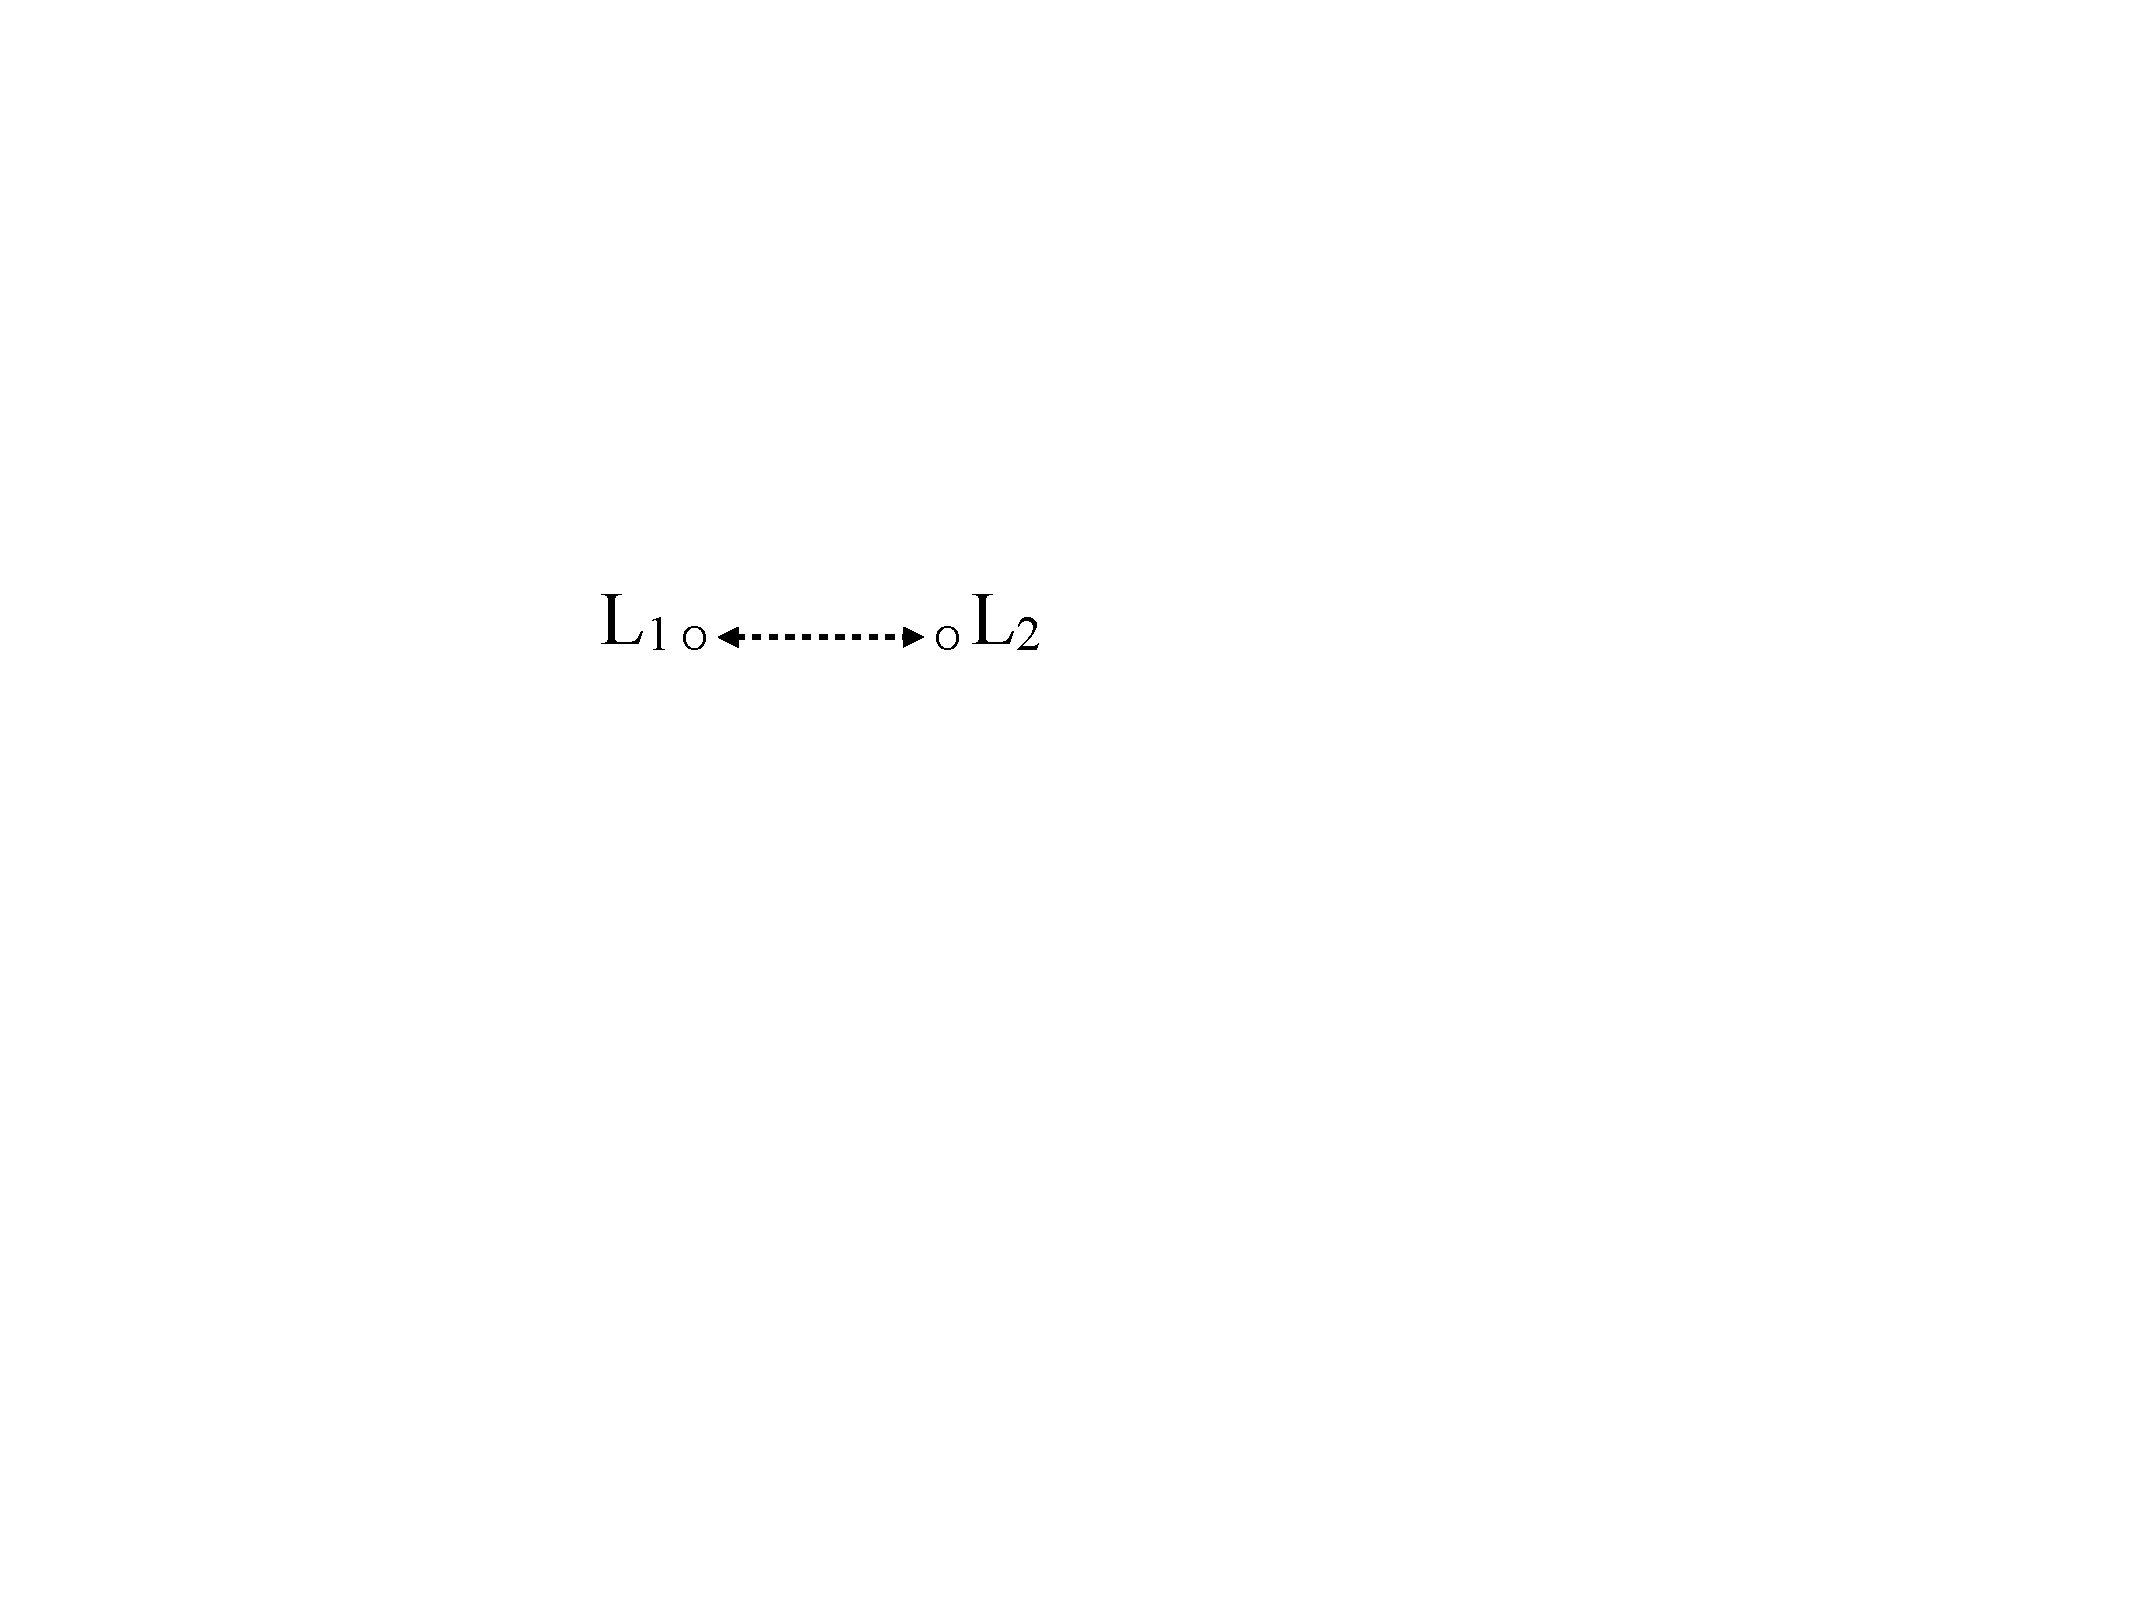
\includegraphics[width=2.2cm]{Fig/SymbAbbrev/CorefNodes.pdf}} & \phantom{:} & in a syntactic representation, indicates that the nodes L\tsub{1} and L\tsub{2} are coreferential -- i.e., they have the same referent \\

L\tsub{1}\thinspace\syntRel{Dep}\thinspace{}L\tsub{2} & \phantom{:} & L\tsub{2} semantically\slashs{}syntactically depends on L\tsub{1} by semantic\slashs{}syntactic dependency \textbf{\textsf{Dep}} \\

L\thinspace\lexRel{\lf{LexRel}}\thinspace{}L′ & \phantom{:} & L′ is the target of the  lexical relation \lf{LexRel} originating from L \\

\idiom{L\tsub{1} ... L\tsub{n}} & \phantom{:} & idiom -- e.g., \idiom{\textit{put the cart before the horse}} \\

\tld & \phantom{:} & the lexical unit under description in a given formula -- e.g., \lfappl{Real\tsub{1}}{\textit{bicycle}} = \textit{ride} \lfgp{\textsc{art} \tld} \\

\suffixsplit & \phantom{:} & \lfgp{in a Russian wordform} boundary between a morphological stem and a suffix\index[notion]{suffix} -- e.g., \textit{sobak\suffixsplit{}a} `dog-\textsc{sg.nom}' \\

\onewdf & \phantom{:} & graphical connector for segments of one wordform that is traditionally spelled as several words -- e.g. \textit{at\onewdf{}last} \\

`\textsigma' & \phantom{:} & a given meaning \\

\sigmaF\ & \phantom{:} & meaning of the lexical function \lf{f} \\

`\myuline{\textsigma}' & \phantom{:} & semanteme that is communicatively dominant in a semantic structure \\

`\tsub{---}' & \phantom{:} & empty actant slot in a semantic structure \\

\textOmega & \phantom{:} & external participant of the situation denoted by L (i.e., a participant that is not expressed as one of L's semantic actants) \\

Ø & \phantom{:} & zero sign \\[2pt]

\multicolumn{3}{l}{In the list of an LF application values (\textit{Val}):} \\*


\textit{Val\tsub{1}}\textbf{;} \textit{Val\tsub{2}} &  & there is a notable semantic difference between \textit{Val\tsub{1}} and \textit{Val\tsub{2}} \\

\textit{Val\tsub{1}} \textbf{<} \textit{Val\tsub{2}} &  & \textit{Val\tsub{2}} is semantically `more' than \textit{Val\tsub{1}}; the left and right scopes of ``<'' can be limited by the ``;'' symbol \\

\fused\textit{Val} &  & \textit{Val} is a fused value element (for a syntagmatic LF) \\*

\textit{Val} \lfgp{GP} & & GP is the government pattern of \textit{Val} -- e.g., \lfappl{Oper\tsub{1}}{\textit{supremacy}} = \textit{detain} \lfgp{\textsc{art} \tld} \\ [-12pt]

\end{longtable}
\endgroup

\noindent
\begingroup
\setlength{\tabcolsep}{2.5pt}
\setlength\extrarowheight{3pt}
\small
\begin{longtable}{ l l >{\raggedright\arraybackslash}p{9cm} }

\multicolumn{3}{l}{{\large \textbf{Special font formats}}} \\*[6pt]

\textsc{small capitals} & \phantom{:} &  lexical unit supplied, when needed, with its lexicographic number -- e.g., the lexeme \textsc{step}\tsub{(V)}\sensenum{I.1} and the idiom \idiom{\textsc{blow the whistle}} \\

\lf{monospace font} & \phantom{:} & lexical function's name -- e.g., \lf{Syn}, \lf{A\tsub{1}}, ... \\

\notion{italicized sans serif font} & \phantom{:} & important notion, when first introduced -- e.g., \notion{idiom} \\*

\uslabel{small bold sans serif font} & \phantom{:} & usage label -- e.g., \uslabel{archaic}, \uslabel{child language}, \uslabel{colloquial}, ...
% Label labels used in the book
% archaic
% child language
% colloquial
% dated
% formal
% informal
% literary
% offensive
% Quebec
% slang
% specialized
% vulgar

\end{longtable}
\endgroup

\noindent
Russian examples are in international scientific transliteration\index[notion]{transliteration}; it is as follows:

\begin{center}
\small
\noindent
\renewcommand*{\arraystretch}{1.2}
\setlength{\tabcolsep}{1.5pt}
\begin{tabular}{ l c l c l c l c l c l c l c l c l c l c l c l }
\midrule

Aa &---& Аа
&\phantom{.....}& Ëë &---& Ёё
&\phantom{.....}& Ja ja &---& Яя
&\phantom{.....}& Oo &---& Оо
&\phantom{.....}& Tt &---& Тт
&\phantom{.....}& \v{Z}\v{z} &---& Жж \\

Bb &---& Бб
& & Èè &---& Ээ
& & Ju ju &---& Юю
& & Pp &---& Пп
& & Uu &---& Уу
& & \palat\ &---& Ьь \\

Cc &---& Цц
& & Ff &---& Фф
& & Kk &---& Кк
& & Rr &---& Рр
& & Vv &---& Вв
& & \palat\palat\ &---& Ъъ \\

\v{C}\v{c} &---& Чч
& & Gg &---& Гг
& & Ll &---& Лл
& & Ss &---& Сс
& & Xx &---& Хх
& & & & \\

Dd &---& Дд
& & Ii &---& Ии
& & Mm &---& Мм
& & \v{S}\v{s} &---& Шш
& & Yy &---& Ыы
& & & & \\

Ee &---& Ее
& & Jj &---& Йй
& & Nn &---& Нн
& & \v{S}\v{c}, \v{s}\v{c} &---& Щщ
& & Zz &---& Зз
& & & & \\

\midrule
\end{tabular}
\end{center}

\clearpage{\pagestyle{empty}\cleardoublepage}

